\documentclass[preprint,5p,times,onecolumn]{article}
\usepackage{graphicx}
\usepackage{amsmath, amssymb}
\usepackage{amsthm}
\usepackage{multirow}
\usepackage{stmaryrd}

\title{Multi-Tesellation for Forman Gradient}

\author{Iuricich Federico$^{1}$ \\
         $^1$Department of Computer Science, University of Genova, Italy.
         }


\begin{document}


\section{Introduction}

The Multi-Tesellation for Forman Gradient (MTFG) is a multiresolution model encoding varius representations for a scalar field, defined on a simplicial 2-complex, both from the geometrical and topological point of view.
The Multiresolution model is encoded as a Direct Acyclic Graph (DAG). 

\noindent
The root of the DAG contains:
\begin{itemize}
	\item the base complex encoded through the IA data structure \cite{Niel97}
	\item a Forman Gradient defined on such complex encoded through the compact representetion described in \cite{weiss13} which requires only 2 bytes per top simplex.
\end{itemize}

Nodes of the DAG represents updates which are geometrical or topological. Geometrical updates are the undo of an edge-contraction \cite{Dey13}, that we will call edge-expansion. An edge-expansion introduces at most two triangles, tree edges and a new vertex in the simplicial complex. A topological refinement defines two simplexes as critical and can be considered as an undo of a removal operator \cite{Comi11}.


\section{MTFG, required items}
\label{sec:build}

In this Section we will describe the steps required to build up a MTFG starting from a simplicial complex given in input. As first step, the simplicial complex $\Sigma$ is encoded using the IA data structure which ecplicitly represents only the vertices $V$ and the triangles $T$. For each vertex its coordinates are stored as well as one of its incident triangles. For each triangle instead, we store the three vertices on its boundary and the adjacent triangles (working with manifold meshes they will be at most one for each boundary edge).\\

Then, the Forman Gradient $F$ is computed on $\Sigma$ using the algorithm described in \cite{Robin11}. Following the encoding described in \cite{weiss13} $F$ will be stored as a set of gradient configurations, one for each triangle in $T$.
Once the simplicial complex and the corresponding Forman gradient are properly stored they are simplified as much as possible in order to obtain a coarser simplicial complex and its corresponding Forman gradient which will become the base complex $\Sigma_B$ stored in the DAG root.

\subsection{Edge-collapse}
And edge-collapse $collapse(v_1,v_2)$ is a well known simplification operation for simplicial complexes which deletes an edge collapsing one of its vertices in the other one, first vertex is deleted as well.
According to the notation showed in Figure \ref{fig:notation}(a) we will indicate with:

\begin{itemize}
	\item $v_1$ the vertex that will be deleted by the edge-collapse,
	\item $v_2$ the vertex that will survive to the edge-collapse,
	\item $e = (v_1,v_2)$ the edge to collapse,
	\item $t^{left}$ the triangle on the left of $e$ to delete,
	\item $t^{right}$ the triangle on the right of $e$ to delete,
	\item $v_3^{left}$ and $v_3^{right}$ the vertices in $t^{left}$ and $t^{right}$, respectively, different from $v_1$ and $v_2$,
	\item $t_1^{left}$ and $t_1^{right}$ the triangles adjacent to $t^{left}$ and $t^{right}$, respectively, on the edge opposite to $v_2$,
	\item $t_2^{left}$ and $t_2^{right}$ the triangles adjacent to $t^{left}$ and $t^{right}$, respectively, on the edge opposite to $v_1$. 
\end{itemize}

Even if an edge collapse can be performed on any edge of $\Sigma$ we want to mantain two invariants across our simplification process.
Each simplification has to be {\em homology-preserving} and must not produce {\em invalid gradient configurations}.

\paragraph{Homology-preserving edge collapse}
In general an edge-collapse is not guaranteed to preserve the homology of the simplicial complex on which it is applied. This is a well studied problem in literature \cite{Dey13} and in our implementation we use a variant of the so called {\em Link Condition} described in \cite{Dey13} for a 2-manifold simplicial complex. We extract all the vertices adjacent to $v_1$ and $v_2$, if the size of this two sets is equal or lower than two, the link condition is mantained and the edge collapse is homology-preserving.

\paragraph{Valid Gradient configuration} 
Second fundamental invariant required is the validity of $F$. Removing simplexes from $\Sigma$ we have to modify $F$ accordingly in the neighborhood of the edge collapsed. The key idea of a gradient update is to locally modify $F$ not generating new critical simplexes and mantaining the gradient flow. To guarantee this, we have to specify some preconditions for the gradient in the neighborhood of the edge deleted. The edge collapse is applicable if:

\begin{itemize}
	\item $t^{left}$ and $t^{right}$ are not critical,
	\item all the edges on $t^{left}$ and $t^{right}$ are not critical,
	\item $v_1$ has more than three incident triangles,
	\item $v_1$ is paired with the edge $e$ in $F$,
	\item $v_3^{left}$ is not paired in $F$ with the edge $(v_3^{left}, v_1)$,
	\item $v_3^{right}$ is not paired in $F$ with the edge $(v_3^{right}, v_1)$.\\
\end{itemize}


\begin{figure}
	\begin{tabular}{c c c}
		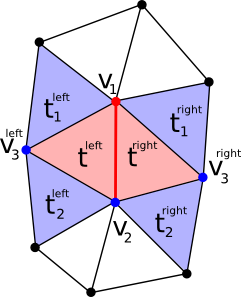
\includegraphics[width=0.33\linewidth]{images/before_edge_collapse} &
		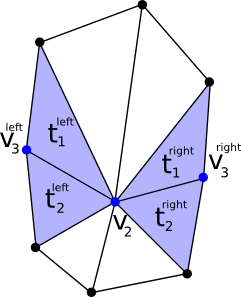
\includegraphics[width=0.33\linewidth]{images/after_edge_collapse} &
		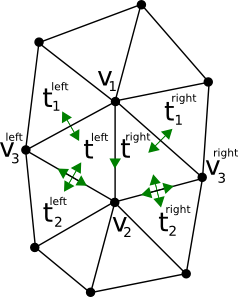
\includegraphics[width=0.33\linewidth]{images/gradient_conf} \\
		(a) & (b) & (c) \\
	\end{tabular}
	\label{fig:notation}
	\caption{In (a) are shown the simplexes involved in a edge-collapse. In (b) the result of the edge collapse and in (c) are shown the gradient arrows (green) that are lecit for the edge-collapse.}
\end{figure}

In Figure \ref{fig:notation}(c) we show all the possible gradient arrows that can appear in the neighborhood of an edge-collapse. Gradient arrows not showed in the figure are pairing simplexes not involved in the edge collapse or are invalid arrows for the collapse operation. 

The edge-collapse applied on the edge $e$ simplify the simplicial complex locally. As showed in Figure \ref{fig:notation}(b) it deletes the edge $e$ collapsing vertex $v_1$ in $v_2$. Triangles $t^{left}$ and $t^{right}$ are deleted as well. As a consequence, 

\begin{itemize}
	\item $t_1^{left}$ become adjacent to $t_2^{left}$ (update TT relation)
	\item $t_1^{right}$ become adjacent to $t_2^{right}$ (update TT relation)
	\item all the triangles incident in $v_1$ switch vertex $v_1$ with $v_2$ (update TV relation)
	\item if $v_3^{left}$ or $v_2$ were storing $t^{left}$ as incident triangle, it is switched with $t_1^{left}$ or $t_2^{left}$ (update VT* relation)
	\item if $v_3^{right}$ or $v_2$ were storing $t^{right}$ as incident triangle, it is changed with $t_1^{right}$ or $t_2^{right}$ (update VT* relation).
\end{itemize}

Thanks to the precoditions, the Forman gradient has to be updated only on a limited number of simplexes. We have to update the gradient codified in $t_1^{left}$ and $t_1^{right}$ in the worst case. Since the updates required are simmetrical on the left and on the right part, respect to the collapsed edge, we will describe them for the left side only.

The updates on $F$ depend on the edges $(v_3^{left},v2)$ and $(v_3^{left},v1)$. If these edge are both paired with a triangle then the edge-collapse require no updates on $F$, (see Figure \ref{fig:arrows}(a) and \ref{fig:arrows}(b)). Otherwise, if the edge $(v_3^{left},v1)$ is paired with a vertex ($v_1$ or $v_3^{left}$ does not matter) this gradient pair must be updated in the graient codified in $t_1^{left}$, (see Figure \ref{fig:arrows}(c) and \ref{fig:arrows}(d)).


\begin{figure}
	\centering
	\begin{tabular}{c c c c}
		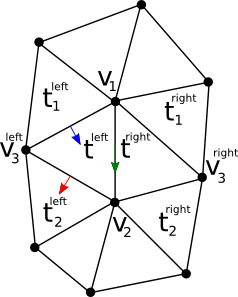
\includegraphics[width=0.22\linewidth]{images/gradient_left_before} &
		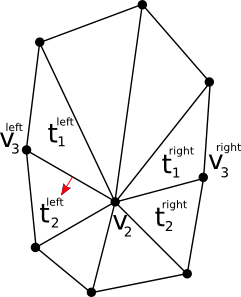
\includegraphics[width=0.22\linewidth]{images/gradient_left_after} &
		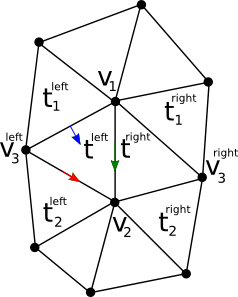
\includegraphics[width=0.22\linewidth]{images/gradient_left_before2} &
		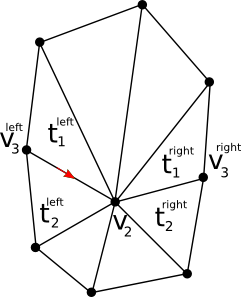
\includegraphics[width=0.22\linewidth]{images/gradient_left_after2} \\
		(a) & (b) & (c) & (d) \\
	\end{tabular}
	\label{fig:arrows}
	\caption{In (a) and (b) is shown a gradient configuration that does not require an update of $F$ during an edge collapse. Triangle $t_1^{left}$ has an arrow pointing the adjacent triangle before (blue arrow in (a)) and after (red arrow in (b)) the edge collapse. On the countrary, if the gradient configuration is different (in (c)) it losts the arrow pointing the adjacent triangle after the edge collapse (see (d)) }
\end{figure}

In the implementation, are performed all the updates on the gradient first, then the two triangles $t^{left}$ and $t^{right}$ and the vertex $v_1$ are removed and the IA data structure is modified updating the new adjacencies between triangles.


\subsection{Edge-collapse by batch}
Edge-collapse simplifications are the first tool we use to reduce the resolution of $\Sigma$ and, consequently, its storage cost. Our goal is to apply as mush edge-collapses as possible and, at the same time, to distrubute them throughout the dataset in order to decrease the resolution uniformly. To achieve this result, we use a simplification algorithm that we will call by batch. Given $\Sigma$ we enqueue all the performable edge-collapses in a priority queue in ascending order of edge lenght. The first collapse is performed and all the vertices adjacent to the removed one are marked as visited. Then, a collapse is performed only if the two vertices on the edge are not yet visited. Once the priority queue is empty a new one is built with all the new performable edge-collapse and all the vertices are marked has unvisited. The edge-collapse by batch ends when no more collapses are performable.\\

The definition of a simplification algorithm is a fundamental step for the construction of a multiresolution-model. As discussed in other works \cite{Comi13}, different simplification algorithms infer different properties on the DAG that will codify the multiresolution model. For the MTFG we have chosen a batch simplification maximizing the number of independent simplifiations (and thus of independent refinements) in order to maximize the number of representations that can be extracted.



\subsection{Topological simplification}
The second type of simplifications we want to perform on the scalar field are topological. We will use two types of simplification operators defined in \cite{Comi11} to reduce the number of critical points in the scalar field, these operators are called $removal_{i,i+1}$ and $removal_{i,i-1}$. A removal operator remove two critical simplexes from a Forman gradient changing locally the flow of $F$. We will not discuss here the updates that this operator causes on the scalar field but we will describe (briefly) only the updates in terms of Forman gradient.\\

Given a Forman gradient $F$ and a $removal_{i,i+1}(q,p,p')$, where $q$ is a critical $i$-simplex connected with the two critical $(i+1)$-simplexes $p$ and $p'$ by two single $(i+1)$-paths on $F$, we call $F'$ the Forman gradient obtained applying $removal_{i,i+1}(q,p,p')$ on $F$. 

To obtain $F'$ critical simplexes $q$ and $p$ are removed by the set of critical simplexes and the (i+1)-path connecting $p$ to $q$ is reversed. Formally, given a path

$$ p = \tau; (\sigma_1, \tau_1); (\sigma_2, \tau_2); ... ; (\sigma_n, \tau_n); \sigma = q $$

where $(\sigma_i, \tau_i)$ is a pair in $F$ and $\sigma_i$ is a simplex on the boundary of $\tau_{i-1}$, we will obtain the following gradient path

$$(\sigma_1, \tau); (\sigma_2, \tau_1); ... ;  (\sigma_n, \tau_{n-1}); (\sigma, \tau_n)  $$.

This kind of simplifications cause an update of the gradient encoded only while no updates are performed on the simplicial complex (IA data structure). An example of the updates performed on the gradient are shown in Figure \ref{fig:grad_simpl} for a 2-path (a) and (b) and for a 1-path (c) and (d).

\begin{figure}
	\begin{tabular}{c c}
		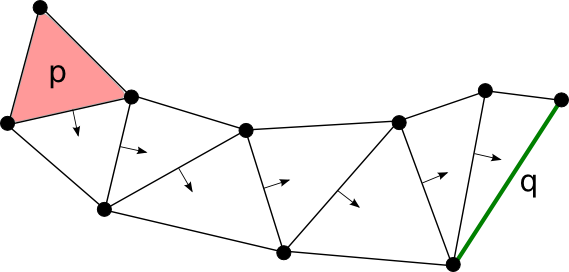
\includegraphics[width=0.45\linewidth]{images/twopath-critical} &
		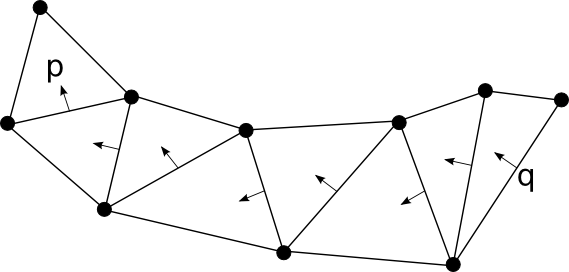
\includegraphics[width=0.45\linewidth]{images/twopath} \\
		(a) & (b) \\
		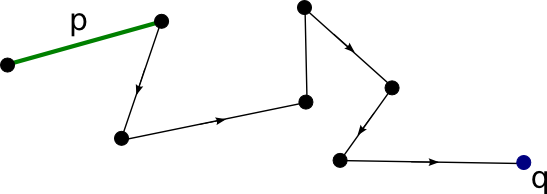
\includegraphics[width=0.45\linewidth]{images/onepath-critical} &
		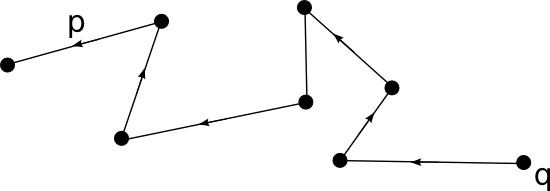
\includegraphics[width=0.45\linewidth]{images/onepath} \\
		(c) & (d) \\
	\end{tabular}
	\label{fig:grad_simpl}
	\caption{In (a) an example of a 2-path connecting a critical triangle with a critical edge. In (b) the 2-path is inverted deleting the two critical simplexes. In a similar fashio in (c) a 1-path is shown and in (d) the same 1-path is inverted deleting the critical vertex and the critical edge.}
\end{figure}


\subsection{Topological simplification by batch}
Similarly to the geometrical simplifications, we want to perform as much topological simplifications as possible distributing them throughout the dataset. To achieve this result we use a support data structure encoding the incidence graph (IG) of the critical points of the scalar field. We will not described the IG in details. A complete description can be found in \cite{Comi13} where is illustrated how the IG provides a compact representation of the scalar field as well as a representation for the incidence relations between the cells of the Morse complexes.

The IG is extracted from $F$ and is kept up to date during the undergoing of topological simplifications. The simplification algorithm that we use is the same used in \cite{Comi11a}. At the beginning a priority queue is built with all the valid topological simplifications performable. When a simplification is performed all the nodes involved are marked as visited and no other simplification will be performed on them until other simplifications are available. When the priority queue is empty it is refilled with new simplifiations unmarking all the nodes in the IG, and when no more simplifications are available the algorithm ends.


\subsection{Building the root of the MTFG}
Building an $MTFG$ from a simplicial complex $\Sigma$ is a procedure that alternates geometrical and topological simplification algorithms. As first step the incidence graph $IG$ is computed on $F$.
Then all the performable edge-collapses are executed until all the edges present an invalid configuration to be collapsed. Thus the queue of the topological simplifications is prepared and a percentage of all the possible topological simplifications is performed. This percentage can be a user-defined parameter. We have fixed this parameter based on the persistence range among all the possible simplifications. At each iteration are performed all the simplifications having persistence value lower or equal than the 10\% of the maximum persistence value. Performing some topological simplifications will unlock new edge-collapses (since some critical simplexes are removed and some arrows are flipped). This interchange of geometrical and topological simplifications continues until no more simplifications are available.\\

All the information regarding the simplifications executed are stored in two lists, one for the geometrical and one for the topological. These will be the chunk used to build up the DAG structure of the MTFG. The root of our DAG is built, at this point, storing the base simplicial complex $\Sigma_B$ obtained performing all the edge-collapse and the corresponding base Forman gradient $F_B$.


\section{Building the MTFG and its storage cost}
\label{sec:store}

Once all the simplifications have been performed and stored build up a MTFG corresponds to create the DAG nodes (one for each simplification) connecting them accordingly to a dependency relation. In this Section we will describe the two types of DAG nodes, {\em geometrical DAG node} ($node_{geom}$) and {\em geoemtrical DAG node} ($node_{topo}$), and we will describe the dependency relations among them.
\subsection{Geometrical DAG Node}

A geometrical DAG node encodes the edge expansion refinement, undo of an edge-collapse $collapse(v_2,v_1)$. A geometrical DAG node $node_{geom}$ representing an edge expansion encapsulates:

\begin{itemize}
	\item a vector $vv$ of vertices adjacent to $v_2$ when the $collapse(v_2,v_1)$ was applied,
	\item the coordinates of the new vertex inserted $v_2$
	\item an integer $v$ indicanting the vertex $v_1$ that will be on the boudnary of the new edge with $v_2$,
	\item a set of $node_{geom}$ from which this operation depends (see Section \ref{sec:dep}).
	\item a boolean value indicating wether the expansion has been applied or not.
\end{itemize}

Vertices in $vv$ are stored in a precise orded such that in the firsts two positions of the vector will be stored the two vertices $v_3^{left}$ and $v_3^{right}$ (see Figure \ref{fig:notation}(a)).  
Memory occupied by vertex $v_2$ instead is used differently before and after the expansion is executed. If the expansion is not yet applied integer $v$ indicates the index of vertex $v_1$. After the expansion, its value will be replaced with the index of the new vertex $v_1$. This is an implementation trick to have an access (with complexity O(1)) to a vertex during the extraction of the front complex $\Sigma'$\\

\paragraph{Implementation explanation}
All the indices of a vertex in the MTFG are store as signed integers. We have to distinghuish between vertices codified in the base complex $\Sigma_B$ and vertices that will be introduced by some $node_{geom}$. To do this, we store all the $node_{geom}$ in consecutive memory cells. Then, we distinguish among this two kind of vertices representing them as:

\begin{itemize}
	\item a negative integer $-i$, if the index correspond to the $i$-th vertex in $\Sigma_B$,
	\item a positive integer $i$, if the index corresponds to the vertex introduced by the $i$-th $node_{geom}$. If the expansion codified in $node_{geom}$ has been applied, $v$ represent the actual index of the vertex in the front complex $\Sigma'$.
\end{itemize}

%bisogna dire cosa si fa qui
The refinement will reintroduce a vertex $v_2$ as well as a new edge $e$ and the two incident triangles $t^{left}$ and $t^{right}$. (See Figure \ref{fig:geom-insert}(b)).
The updates required on the IA data structure are:
\begin{itemize}
	\item add a new vertex $v_1$ in the set of vertices,
	\item add a new triangle $t^{left}$ composed by the three vertices $(v_1,v_2,v_3^{left})$
	\item add a new triangle $t^{right}$ composed by the three vertices $(v_1,v_2,v_3^{right})$
	\item set the adjacenct triangles of $t^{left}$ as $(t_1^{left}, t_2^{left}, t^{right})$
    	\item set the adjacenct triangles of $t^{right}$ as $(t_1^{right}, t_2^{right}, t^{left})$
	\item all the triangles between $t^{left}$ and $t^{right}$ (visited in cw order) get $v_1$ as incident vertex instead of $v_2$.
\end{itemize}

\begin{figure}
	\begin{tabular}{c c c c}
		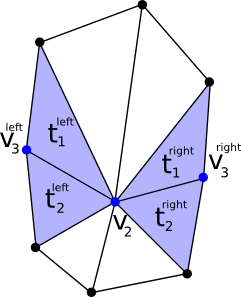
\includegraphics[width=0.22\linewidth]{images/after_edge_collapse} &
		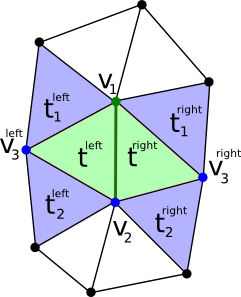
\includegraphics[width=0.22\linewidth]{images/after_edge_refinement} &
		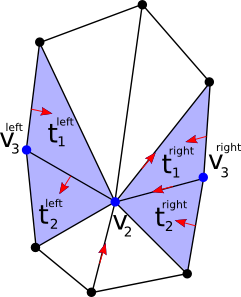
\includegraphics[width=0.22\linewidth]{images/gradient_before_refinement} &
		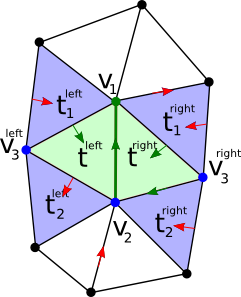
\includegraphics[width=0.22\linewidth]{images/gradient_after_refinement} \\
		(a) & (b) & (c) & (d) \\
	\end{tabular}
	\label{fig:geom-insert}
	\caption{In (a) is shown a set of simplexes before the edge expansion showed in (b). In (c) and (d) the same edge expansion is illustrated showing the updates required on the Forman gradient with two different configurations on the left and on the right of the introduced edge.}
\end{figure}

Also the front Forman gradient $F'$ has to be modified in the neighborhood of the introduced simplexes. Similarly to the collapse, we can unambiguosly determine how to extend the gradient on the new simplexes simply knowing the gradient defined on the actual simplexes.

Updates required on the front forman gradient $F'$ are the following (as before we will describe the updates only for the left side):
\begin{itemize}
	\item new edge edge $e$ is paired in $F'$ with $v_1$ or $v_2$. If $v_2$ is paired with an edge that will be redirected to $v_1$, than e is paired with $v_2$ otherwise it is paired with $v_1$. (See Figure \ref{fig:geom-insert}(c) and (d))
	\item if edge $(v_3^{left},v_2)$ is paired with $v_2$ or $v_3^{left}$, then edge $(v_3^{left}, v_1)$ is paired with $t^{left}$
	\item if edge $(v_3^{left},v_2)$ is paired with $t_2^{left}$, then edge $(v_3^{left}, v_1)$ is paired with $t^{left}$
	\item if edge $(v_3^{left},v_2)$ is paired with $t_1^{left}$, then edge $(v_3^{left},v_2)$ will be paired with $t^{left}$ and edge $(v_3^{left},v_1)$ will be paired with $t_1^{left}$.
\end{itemize}



\subsection{Topological DAG Node}

A topological DAG node encodes the refinement applicable on an intermediate Forman gradient $F'$, undo of a removal. A topological DAG node $node_{topo}$ representing a refinement encapsulates:

\begin{itemize}
	\item the set of vertex indices indicating the simplex that will be critical (a triangle or a point)
	\item the pair of vertex indices indicating the edge that will be critical
	\item a set of $node_{topo}$ from which this operation depends (see Section \ref{sec:dep}).
	\item a set of $node_{geom}$ from which this opeartion depends (see Section \ref{sec:dep})
\end{itemize}

As undo of a removal the refinement introduce two critical simplexes reversing the gradient arrows in order to create a path from the simplex of higher dimension to the simplex of lower dimension. Is not necessary to codify the path complitely since, knowing the correct starting simplex the path to reach the ending critical simplex is unique. There is no need to store any other information on the other critical simplexes in the neighborhood, required from the operation, but they are implicitly encoded in the dependency relations 

To follow a unique path we always need to start from the critical simplex of higher dimension. We will describe here the two different paths followed in case the operation is an $insert_{i,i+1}$ or an $insert_{i,i-1}$.

\paragraph{$insert_{i,i+1}$} 
In the case of 2-complexes this will correspond to the introduction of a critical edge $e$ and a critical triangle $t$, saddle and maximumum critical points respectively. The triangle $t$ is identified and the edge $e_1$ with which is paired is stored. Then $t$ is set as critical and the $e_1$ is used to navigate to the adjacent triangle of $t$, $t_1$. At this point, having $e_1$ and $t_1$ we proceed recursively:

\begin{itemize}
	\item $e_t$ is the pair of $t_1$ in $F'$
	\item we make a new pair in $F'$ $(e_1,t_1)$
	\item $e_1$ = $e_t$
	\item $t_1$ = adjacent of $t_1$ on edge $e_t$ 
\end{itemize} 

This corresponds to swap the arrows until $e_t$ is equal to $e$. Then, $e_t$ is set as critical and the algorithm ends.


\paragraph{$insert_{i,i-1}$} 
In the case of 2-complexes this will correspond to the introduction of a critical edge $e$ and a critical vertex $v$, saddle and minimum critical points respectively. The critical vertex $v$ is identified and the edge $e_1$ with which is paired is stored. Then $v$ is set as critical and $e_1$ is used to navigate to the adjacent vertex $v_1$. At this point, having $e_1$ and $v_1$ we proceed recursively:

\begin{itemize}
	\item $e_t$ is the pair of $v_1$ in $F'$
	\item we make a new pair in $F'$ $(v_1,e_1)$
	\item $e_1$ = $e_t$
	\item $v_1$ = vertex adjacent of $v_1$ on edge $e_t$ 
\end{itemize} 

This corresponds to swap the arrows until $e_t$ is equal to $e$. Then, $e_t$ is set as critical and the algorithm ends.


\subsection{Dependency relations}
\label{sec:dep}

The dependency relation between two DAG nodes express a constrained order in which two opertions must be performed. We can indentify three types of dependency relations: dependecy between geometrical DAG nodes, dependency between topological DAG nodes and dependency of a topological DAG node from a geometrical DAG node.

\paragraph{Geometrical vs Geometrical}
Intuitively, a geometrical DAG node $n_1$ depends from a geometrical DAG node $n_2$ when $n_2$ introduce a vertex used by $n_1$. In our work we set the dependency based on the set of vertices $vv$ (see Section \ref{sec:store}). So formally, $n_1$ depends from $n_2$ if $n_2$ introduce a vertex present in the set $vv$ of $n_1$.

\paragraph{Topological vs Topological}
Intuitively, a topological DAG node $n_1$ depends from a topological DAG node $n_2$ when $n_2$ introduce a critical simplex that is involved in the neighbrohood of $n_1$. This can be easily noticed considering the operations on the IG instead of on the Forman gradient $F$ (see \cite{Comi13a}). Thus these information are stored during the simplification process, saving, for each node deleted from the IG which DAG represent its deletion. Once the hierarchy is built these information are used to connect the different topological DAG nodes with arcs in the DAG and information on the nodes of the IG are no longer required.

\paragraph{Topoligical vs Geometrical}
Each topological DAG node can be also dependent from a geomtrical DAG node. In particular to execute a topological refinement the two critical simplexes have to exist in the simplicial complex and in particular all the vertices composing them, must be present in $\Sigma'$. We can assure that, if all the vertexes composing the required simplexes, are inside the simplicial complex, then the two critical simplexes are inside the simplicial complex as well.\\

From these set of dependencies we can see that a geometrical refinement is always independent from the topological resolution while a topological refinement is also linked to a specific resolution level for the geometry. This is the reason why, during the simplification step, we always perform as much geometrical simplification as possible while we perform only a subset of the topological operation performable at each operation. This way we can fix the lowst level of resolution required for each topological operation.   

\subsection{Storage cost}

We can estimate the storage cost for the MTFG considering the storage cost of the IA data structure for the simplicial base complex $\Sigma_B$, the storage cost of the base Forman gradient $F_B$, the storage cost for the single DAG nodes and the arcs. We are estimating the storage cost of a pointer as $4byte$.


A geometrical DAG node occupies $4 byte$ for each vertex in $vv$, $32 byte$ for the coordinates of $v_2$ (4 floats), $4 byte$ for vertex $v_1$ and $4 byte$ for each $node_{geom}$ pointer and 1 byte for the boolean. Thus $37 + 4|vv| + 4|node_{geom}|$ byte. \\

A topological DAG node occupies $4 byte$ for each vertex used to indicate the critical simplexes (depending from the opertion we need 6 or 4 vertices), $4 byte$ for each $node_{topo}$ and $4 byte$ for each $node_{geom}$. Thus overestimating the amount of vertices needed, $24 + 4|node_{topo}| + 4|node_{geom}|$, we can overestimate the number of $node_{geom}$ (one for each vertex) and thus it will cost in total
$48 + 4|node_{topo}|$ bytes.\\

The $\Sigma_B$ as described in \cite{Niel97} occupyes $35|V|+24|T|$ where $|V|$ and $|T|$ represent the number of vertices and triangles respectively.




\section{Selective refinement on a MTFG}
\label{sec:query}

Once we have built the $MTFG$ hierarchical structure we can extract representations at different level of details both from the topological and geometrical point of view.
Firstly we have to set the desired resolution from the topological point of view, thus the first input value will be the minimum persistence value desired inside the complex. The topological refinements performed will include also some geometrical refinement since, some of the topological operations will be dependent by some edge-expansion.

Once the desired persistence level is reached, the geometry can be refined as well. In a uniform selective refinement query the minimum persistence and the minimum edge-lenght are set throughout the dataset uniformely.

However, more interesting queries can be performed thanks to the DAG structure of the multiresolution model, we call these queries {\em extraction at variable resolutions}. In this kind of queries different resolutions levels are set, for both the persistence and the edge-lenght values, across the dataset.
For the topological resolution then, two values are given in input, first one indicates the desired resolution inside the region of intereset (a box or a sphere inside the domain) while the second value indicates the desired resolution outside the region of interest. Once the topological resolution has been increased at wish, two new values are given in input to increase the geometrical resolution in a similar fashion.
The region of interest used for the geometrical resolution can be the same used for the topological refinements or a new one. It can also be dependent from topological properties and not be set in a particular region. Given a persistence value $p$, for example, we can increase to resolution $r$ all the simplexes belonging to a Morse cell having persistence value greater or equal than $p$ [not yet implemented].



\bibliography{mm_biblio}
\bibliographystyle{plain}



\end{document}
